\subsection{Styr- och reglersystem}
\label{subsec:styr och regler}
För att styra svävaren samlas acclerometerdata in i realtid på fjärrkontrollen som sedan processeras och omvandlas till styrsignaler som skickas till routern där det även finns plats för ett reglersystem.

\subsubsection{Styrsystem}
Det finns tre olika styralgorithmer för att processera pitch- och rolldata separat. De tre olika styralgorithmerna processerar acclerometerdatan på liknande sätt men med olika matamatiska funktioner, de tre lägena är logaritmisk, exponentionell och linjär. Man kan genom dropdown listor på fjärrkontrollen välja vilken styralgoritm som ska användas. De olika styralgoritmerna utvecklades med hjälp av MATLAB för att sedan implementeras i JAVA på fjärrkontrollen. De olika styralgoritmernas utslag då pitch = 30\degree  då roll går från -45\degree till 45\degree  kan ses i figur~\ref{fig:styralgoritmer}.

\begin{figure}[htbp!]
\centering
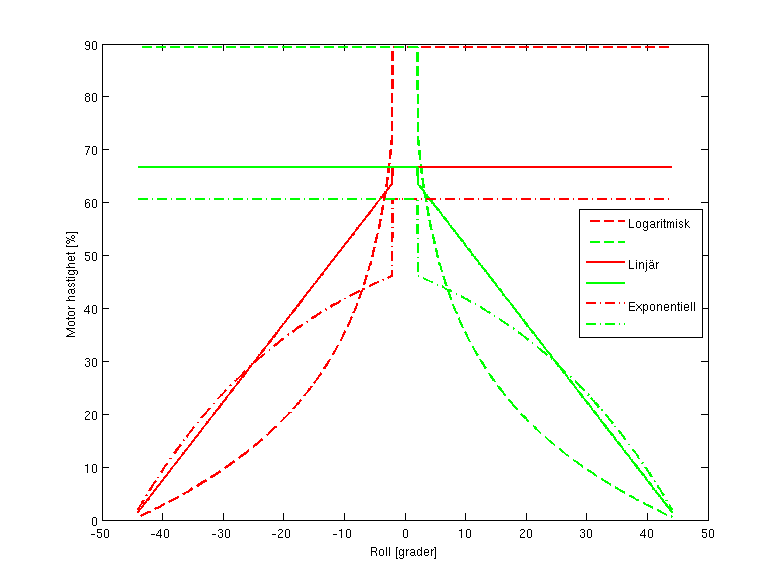
\includegraphics[width=12cm]{../../includes/figures/Styralgoritmer}
\caption{Styralgoritmernas utslag vid pitch = 30\degree då roll = [-45,45].}
\label{fig:styralgoritmer}
\end{figure}

I realiteten märkte föraren dock ingen större skillnad mellan de olika styrlägena. 

\subsubsection{Reglersystem}
Designen av svävaren medförde att hastighet och styrning var starkt korskopplade vilket medför svårigheter då en regulator ska implementeras. Grundlig efterforskning gjordes och det bestämdes att ramverket ACADO skulle användas för att implementera en regulator till svävaren då ramverket kunde autogenerera kod för mer komplexa regulatorer. Detta visade sig vara svårare än förutspått och ramverket krävde även mer minne än vad som fanns tillgängligt. Dessa bakslag medförde att reglersystemet lades på is för att kunna vidareutvecklas vid ett senare tillfälle.
